\begin{figure}
\begin{center}
    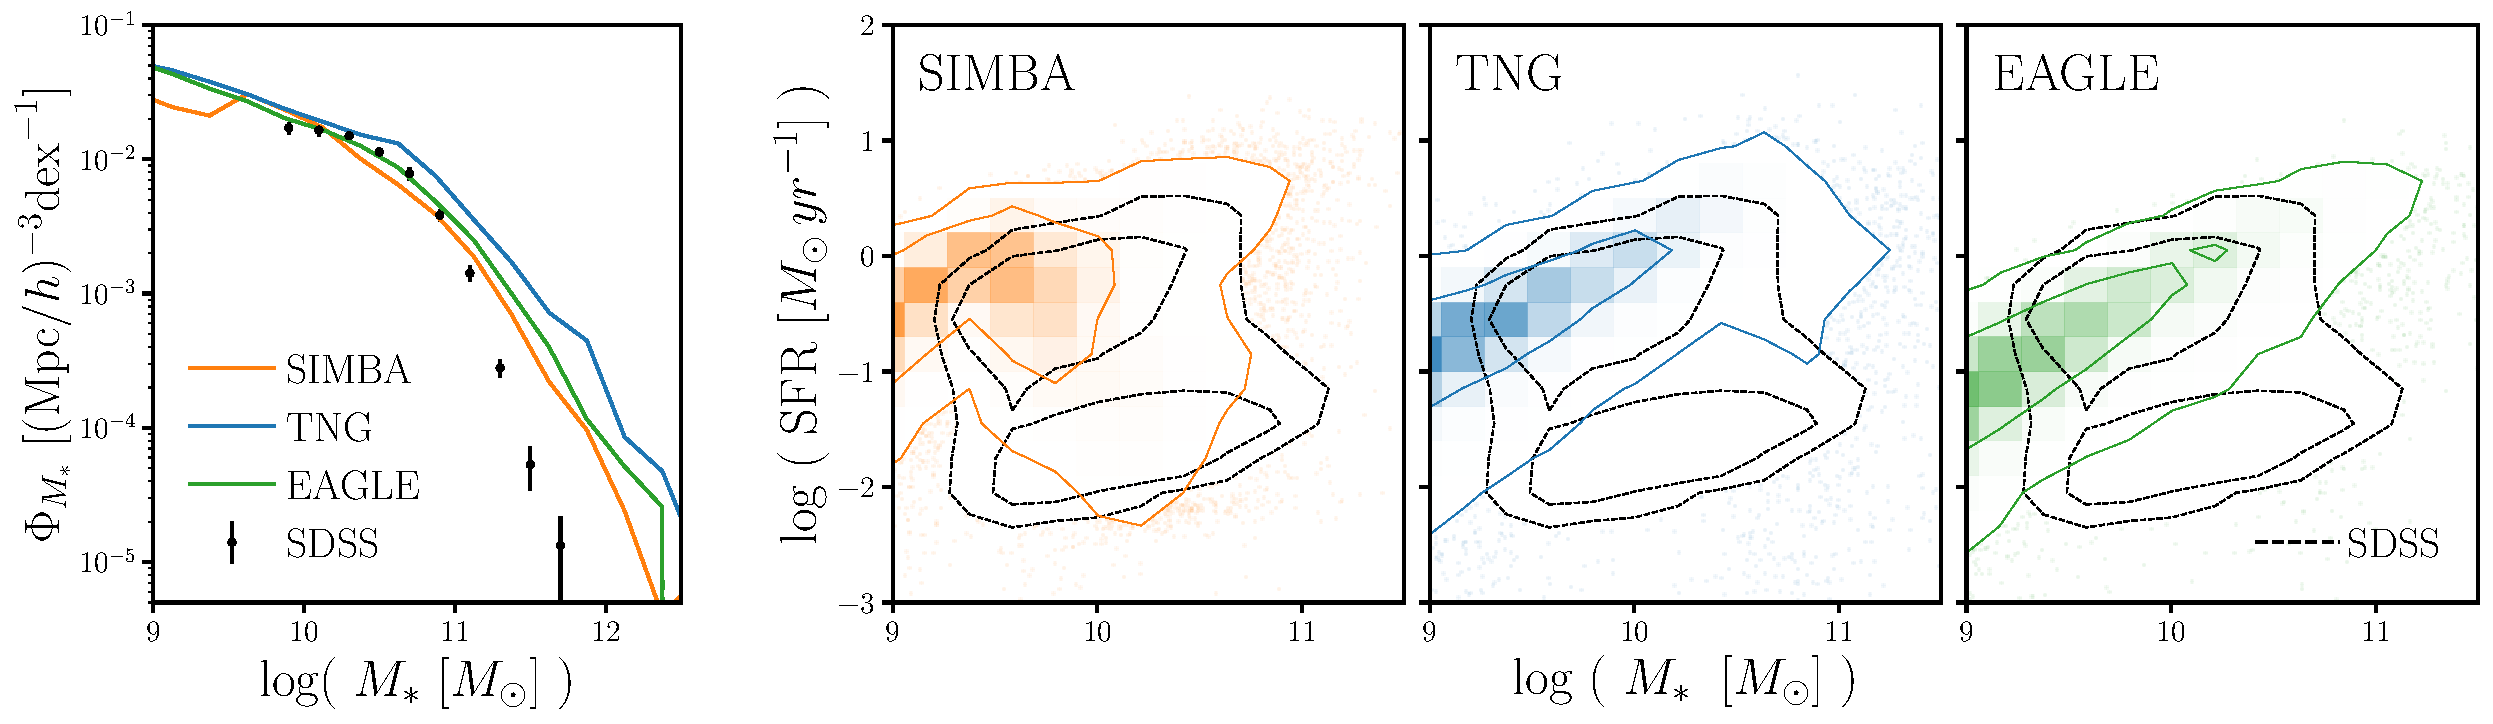
\includegraphics[width=\textwidth]{figs/smf_m_sfr.pdf}
    \caption{\label{fig:smf_msfr}
    The stellar mass functions ($\Phi^{\rm cen}_{M_*}$; left-most panel) and
    $M_*-\sfr$ relation (right panels) of central galaxies from the SIMBA 
    (orange), TNG (blue), and EAGLE (green) simulations. For details on the
    $M_*$ and $\sfr$ of the simulations see Section~\ref{sec:sims}. We also 
    include $\Phi^{\rm cen}_{M_*}$ (black) and the $M_*-\sfr$ relation (black
    dashed) for our SDSS central galaxy sample (Section~\ref{sec:obs}). Uncertainties 
    for the SDSS $\Phi^{\rm cen}_{M_*}$ are derived using jackknife resampling.
    Differences in $\Phi^{\rm cen}_{M_*}$ and the $M_*-\sfr$ relations among
    the simulations highlight how the \emph{hydrodynamical simulations predict
    central galaxies with significantly different the physical properties.}
    }
\end{center}
\end{figure}

\section{Data}\label{sec:sims}
In this paper we apply dust empirical models (DEM) to forward modeled spectral
energy distributions for galaxies in the Illustris TNG, EAGLE, and SIMBA 
cosmological hydrodynamical simulations. Afterwards, we compare the observables
predicted by our DEMs to central galaxies in SDSS DR7 observations. Below, in
the rest of the section, we briefly describe the hydrodynamical simulations 
and the SDSS observations as well as the data we use from them.

In Figure~\ref{fig:smf_msfr}, we present the stellar mass functions ($\Phi^{\rm
cen}_{M_*}$; left-most panel) and $M_*-\sfr$ relations (right panels) for
central galaxies in the SIMBA (ornage), TNG (blue), and EAGLE simulations. We
include, for reference, $\Phi^{\rm cen}_{M_*}$ and the $M_*-\sfr$ relation for
our SDSS central galaxy sample. The uncertainties for the SDSS SMF are derived from
jackknife resampling. 


% also mention that M* and SFR definitions are not consistent for the
% simulations?  
Although we present the SMFs for reference, we do not use
stellar masses throughout the paper since they are inconsistently defined among
simulations and observations. Instead, we compare between the simulations and
SDSS using luminosity, $M_r$, which we consistently forward model and measure
in the simulations. In these comparisons, we restrict ourselves to galaxies
brighter than $M_r < -20$, where our SDSS central galaxy sample is complete. 


\subsection{Illustris TNG} \label{sec:tng}
The Illustris TNG simulation\footnote{\url{https://www.tng-project.org/}}
(hereafter TNG) is a cosmological hydrodynamical simulation of comoving 
volume $(110.7\,\mpc)^3$~\citep{nelson2018,pillepich2018b,springel2018}. It
improves on the original Illustris simulation\footnote{\url{http://www.illustris-project.org}}~(\citealt{vogelsberger2014,genel2014};
public data release by~\citealt{nelson2015}), by including
magneto-hydrodynamics and updated treatments for galactic winds, metal
enrichment, and AGN feedback. Most notably, TNG uses a new implementation for
feedback from SMBH~\citep{weinberger2018}, where feedback energy is injected in
the form of a kinetic AGN-driven wind at low SMBH accretion rates. This new
implementation has been shown to alleviate discrepancies found between the
original Illustris and observations for $> 10^{13-14} M_\odot$ massive halos. 
%TNG has a baryonic mass resolution of $1.4\times10^6M_{\sun}$ \ch{temporal resolution?}.
\todo{details on the following properties that we use in the paper}
\begin{itemize}
    \item SFH
    \item ZH 
    \item stellar mass 
    \item instantaneous SFR
\end{itemize} 

\subsection{EAGLE} \label{sec:eagle} 
In this work, we use L0100Ref of the Virgo Consortium's EAGLE
project\footnote{\url{http://www.eaglesim.org}}, a publicly available suite of
cosmological hydrodynamic simulations~\citep{schaye2015, crain2015,
mcalpine2016}. The simulation has a comoving volume of $(100\,\mpc)^3$ and % baryonic mass resolution of $1.81\times 10^6M_{\sun}$. It 
is simulated with the {\sc Anarchy} code (Dalla Vecchia et al. in prep.; 
see also Appendix A of \citealt{schaye2015}), a modified version of the 
{\sc GADGET-3} code~\citep{springel2005}.
%that includes a conservative pressure-entropy formulation for the smoothed particle hydrodynamics calculation, artificial viscosity, artificial conduction and the time limiter that improve hydrodynamic computation performance. 
It has subgrid models for star formation, stellar mass loss, metal enrichment
and stellar feedback that stochastically inject thermal energy in the ISM as
in~\citep{dallavecchia2012}; the feedback energy from AGN is also added to
surrounding gas stochastically~\citep{Booth2009}. Parameters of the stellar 
feedback and SMBH accretion are calibrated to broadly reproduce the $z=0$ 
stellar mass function and galaxy stellar size-stellar mass relation. Meanwhile, 
the AGN feedback efficiency is calibrated to match the SMBH-galaxy mass relation. 
\todo{details on the following properties that we use in the paper}
\begin{itemize}
    \item SFH
    \item ZH 
    \item stellar mass 
    \item instantaneous SFR
\end{itemize} 

\subsection{SIMBA} \label{sec:simba}
The {\sc Simba} simulation suite~\citep{dave2019}, the successor to {\sc
Mufasa}~\citep{dave2016, dave2017, dave2017a}, is a cosmological hydrodynamical
simulation construted using {\sc Gizmo}, a meshless finite mass hydrodynamics 
code~\citep{hopkins2015a,hopkins2017}. Of the simulations, we use
`m100n1024', which has a box size of $(100\,h^{-1}\,\mpc)^3$ and baryonic 
mass resolution of $1.82 \times 10^7\ M_\odot$. The simulation uses the same
subgrid models as {\sc Mufasa} for $\rm H_2$ based star formation, decoupled
two-phase winds for star formation driven galactic winds, and feedback from 
Type I supernovae and AGB stars. Meanwhile, it uses updated models for AGN
feedback and on-the-fly dust model. {\sc Simba} uses a two-mode SMBH accretion 
model, torque-limited accretion for cold gas~\citep{anglesalcazar2017} and 
Bondi-based accretion for hot gas, and two-mode AGN feedback. %which ejects bipolar kinetic winds with $\sim 10^3 \kms$ for high SMBH accretion rate, and launches winds with increased velocity of $\sim 8000 \kms$ for low SMBH accretion of Eddington ratio below 2 \%.

\todo{details on the following properties that we use in the paper}
\begin{itemize}
    \item SFH
    \item ZH 
    \item stellar mass 
    \item instantaneous SFR
\end{itemize} 

\subsection{Forward Modeling Spectral Energy Distributions} \label{sec:fm} 
\todo{describe how the SED is generated using the SFH and ZHs} 

\subsection{SDSS DR7 Central Galaxies} \label{sec:obs} 
We compare the simulations and models described below
to the observed SDSS central galaxy sample from the \cite{tinker2011} group
catalog. The group catalog, first, selects volume-limited sample of galaxies at
$z \approx 0.04$ with $M_r < -18$ and complete above $M_* > 10^{9.4}
h^{-2}M_\odot$ from the NYU Value-Added Galaxy
Catalog~\citep[VAGC;][]{blanton2005} of SDSS DR7~\citep{abazajian2009}. The
stellar masses are estimated using the $\mathtt{kcorrect}$
code~\citep{blanton2007a} assuming a~\cite{chabrier2003} initial mass
function. 

Central galaxies are then identified using a halo-based group finder that uses
the abundance matching ansatz to iteratively  assign halo masses to groups.
Every group contains one central galaxy, which by definition is the most
massive, and a group can contain $\ge0$ satellites. As with any group finder,
galaxies are misassigned due to projection effects and redshift space
distortions; however, the central galaxy sample has a purity of ${\sim}90\%$
and completeness of ${\sim}95\%$~\citep{tinker2018}. 

\begin{figure}
\begin{center}
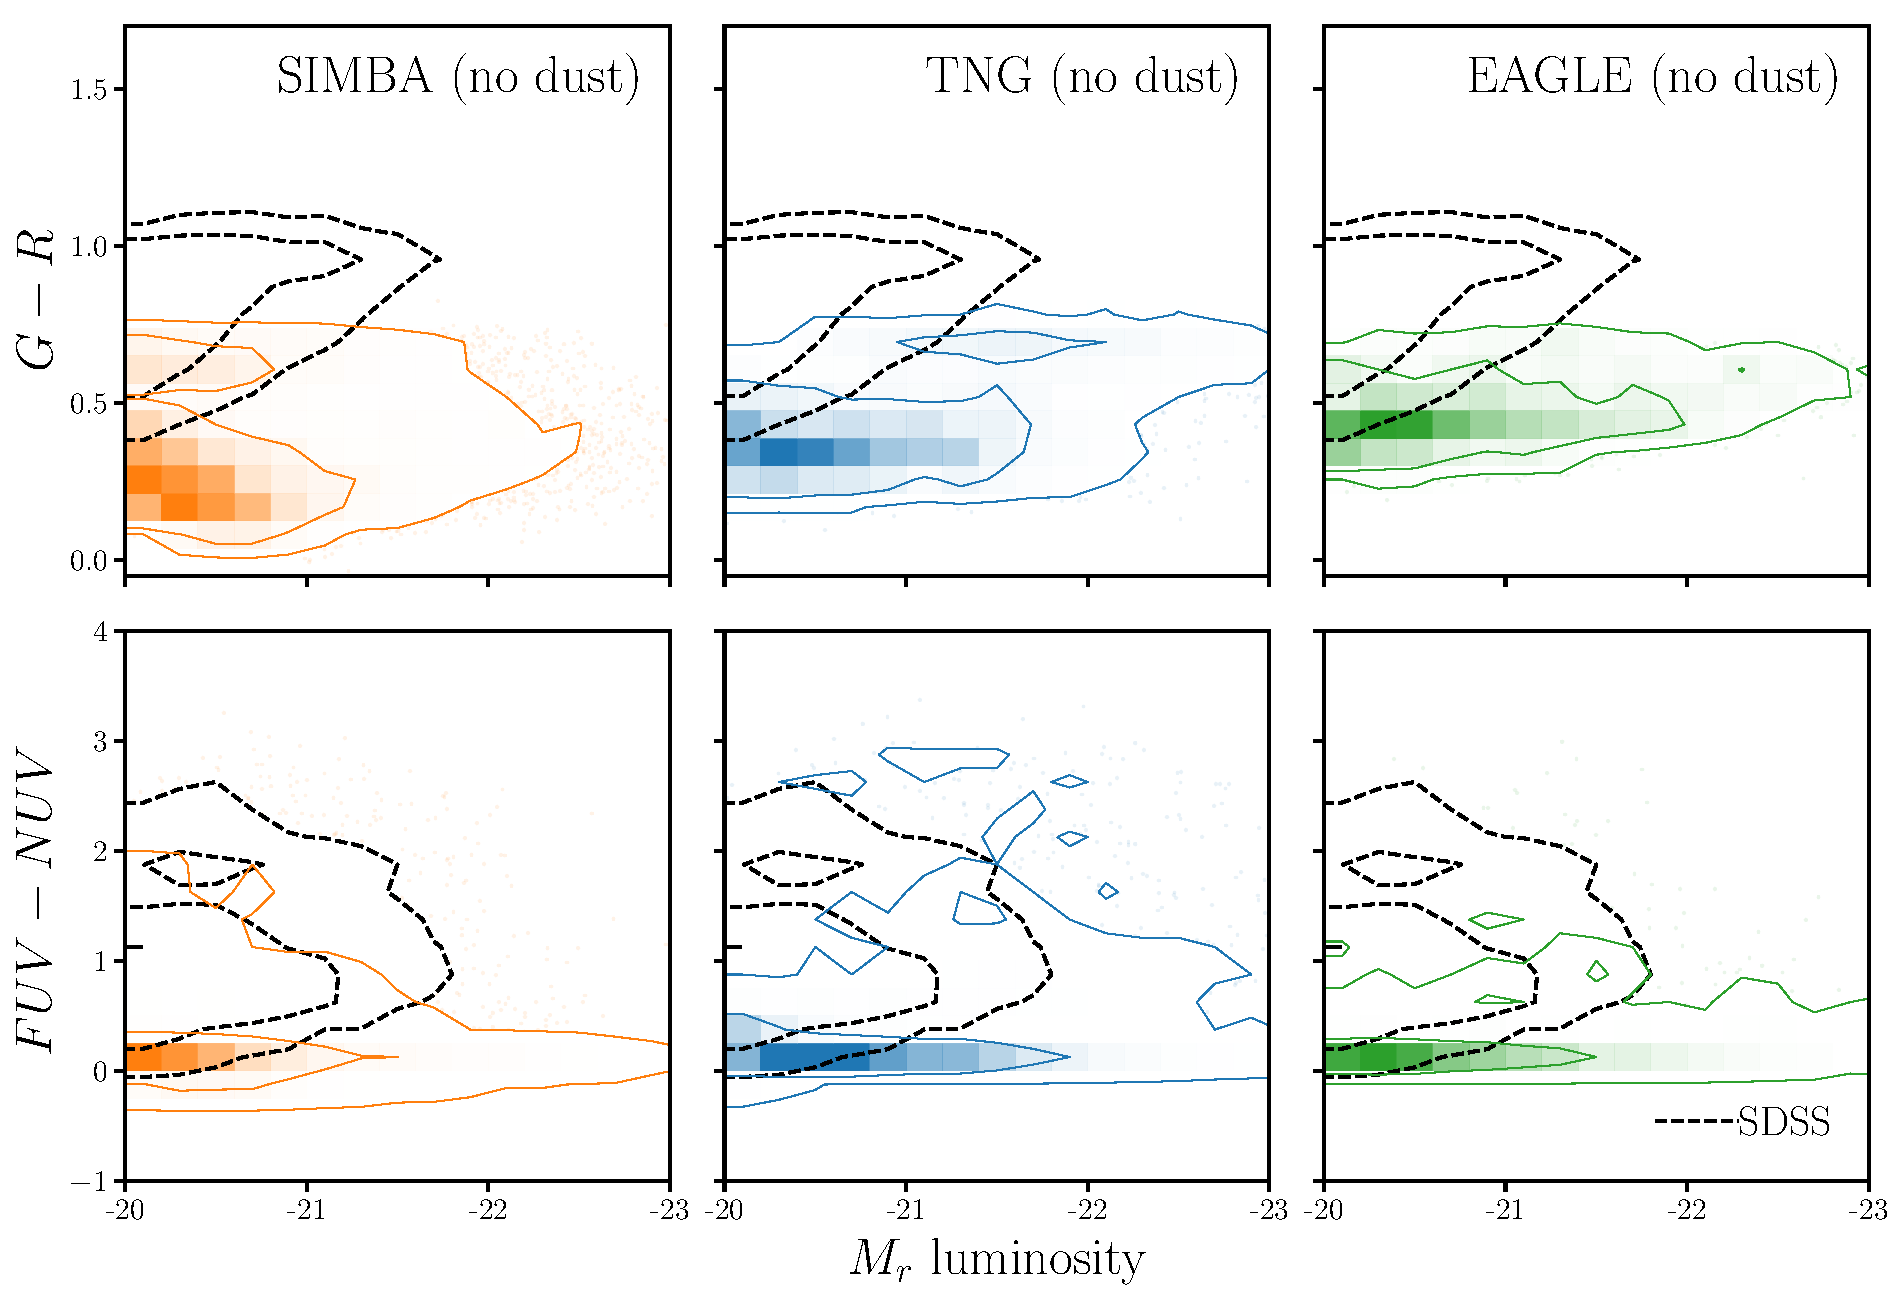
\includegraphics[width=0.9\textwidth]{figs/observables.pdf} 
    \caption{We present the distributions of the main observables used
    throughout the paper for SDSS (left), SIMBA (center), and TNG (right)
    centrals. We do {\em not} include any prescription for dust for the
    simulated galaxies. The top panels
    present the $G-R$ versus $M_r$ color magnitude relations while the bottom
    panels present the $FUV-NUV$ versus $M_r$ relations. The observables for
    the SIMBA and TNG simulated galaxies are derived using forward modeling and
    are therefore consistent with SDSS measurements (Section~\ref{sec:fm}). The
    contours for SIMBA and TNG do not include galaxies with SFR$=0$, which we
    mark separately in black. Despite similar SMFs,  {\em the simulations
    without any dust prescription show stark differences with observations in
    the color-magnitude observable-space.} 
    }
\label{fig:obs}
\end{center}
\end{figure}
